\documentclass[11pt,a4paper]{article}

\usepackage[margin=1.05in]{geometry}
\usepackage{amsmath,amssymb,amsthm}
\usepackage{booktabs}
\usepackage{microtype}
\usepackage{enumitem}
\usepackage{graphicx}
% xcolor must precede tikz, which loads it optionless; colours must precede
% hyperref, which consumes them as option values.
\usepackage[table]{xcolor}
\definecolor{NavyLink}{HTML}{1F4E79}
\definecolor{RuleGrey}{HTML}{888888}
\usepackage{tikz}
\usetikzlibrary{arrows.meta,positioning,decorations.pathmorphing}
\usepackage[colorlinks=true,linkcolor=NavyLink,citecolor=NavyLink,urlcolor=NavyLink]{hyperref}

\newtheorem{observation}{Observation}
\newtheorem{principle}{Principle}

\newcommand{\grad}{\operatorname{grad}}
\newcommand{\curl}{\operatorname{curl}}
\newcommand{\harm}{\operatorname{harm}}
\newcommand{\rank}{\operatorname{rank}}
\newcommand{\tr}{\operatorname{tr}}
\newcommand{\Ph}{P_{\mathrm{h}}}
\newcommand{\Pg}{P_{\mathrm{g}}}
\newcommand{\Pc}{P_{\mathrm{c}}}

\title{\vspace{-1.5em}A Known-Answer Methodology for Calibrating a\\ Harmonic Rankability Certificate}
\author{Meadowlark Bradsher}
\date{August 2026}

\begin{document}
\maketitle

\begin{abstract}
\noindent
A rankability certificate based on the Hodge decomposition of a comparison graph
reports the fraction of comparison ``flow'' that admits no consistent scalar
ordering. Used as a decision procedure it needs a threshold, and the threshold
cannot be read off the mathematics: on finite, noisy, sparsely sampled data a
genuinely rankable criterion still deposits harmonic mass. Calibration therefore
requires knowing what innocent data reads --- which real data cannot tell us,
because real data carries no ground truth.

This document sets out the methodology we applied to that problem: manufacture
comparison data whose Hodge decomposition is known in closed form, validate the
instrument against those known answers, and only then admit a real judge. We
describe the construction, the estimator and its failure modes, the guard
discipline, and the reporting discipline. We give particular weight to three
methodological failures the work exposed --- a constant calibrated on one
topology and silently wrong on another; a guard that passes while the quantity it
protects is wrong by a factor of two; and point estimates quoted for quantities
that vary run to run --- because each was caught only by measurement, and each
generalises beyond this instrument. We close with the principal scope limit the
method establishes: the certificate's threshold is a function of the deployment's
own comparison topology, so there is no universal threshold to ship.
\end{abstract}

\section{The problem}\label{sec:problem}

Let $\mathcal{G}=(V,E)$ be a comparison graph: vertices are items, and an edge
$(i,j)$ with $i<j$ records that the pair was compared. A \emph{flow}
$Y\in\mathbb{R}^{E}$ assigns to each edge the signed advantage of $j$ over $i$.
The HodgeRank construction \cite{jiang2011} decomposes any such flow into three
orthogonal parts,
\begin{equation}
Y \;=\; \underbrace{\grad}_{\in\,\mathrm{im}\,D_0}
      \;+\; \underbrace{\curl}_{\in\,\mathrm{im}\,D_1^{\top}}
      \;+\; \underbrace{\harm}_{\in\,\ker L_1},
\label{eq:hodge}
\end{equation}
where $D_0$ and $D_1$ are the coboundary operators of the simplicial complex on
$\mathcal{G}$ and $L_1 = D_0D_0^{\top} + D_1^{\top}D_1$ is the graph
Helmholtzian. The gradient part is exactly the rankable content: it is the
gradient of a scalar potential, and that potential is the ranking. The harmonic
part is the interesting one. It is globally cyclic --- inconsistent, but with no
triangle to blame --- and its dimension is the first Betti number
$b_1 = |E| - \rank D_0 - \rank D_1$, the number of independent holes. We write
$\Ph$ for the orthogonal projector onto $\ker L_1$; it is the operator every
measurement below is taken through.

A criterion whose comparison flow carries large harmonic mass has no consistent
scalar order, \emph{and} the failure is invisible to any triangle-local
statistic. That makes the harmonic fraction a candidate certificate: a scalar
that says ``this criterion is not rankable, and a triad-consistency check would
not have told you.''

The difficulty is thresholding it. Harmonic mass is not zero for innocent data.
A genuinely rankable criterion, judged noisily, on a sparse graph, deposits some.
So the certificate must be calibrated against the distribution of harmonic mass
under a \emph{true null} --- rankable, but observed the way real data is
observed. Real judgement logs cannot supply that distribution, because we never
know whether a real criterion was rankable to begin with.

\begin{principle}[Calibrate before you judge]
Construct data whose decomposition is known in closed form, establish that the
instrument recovers those known answers, and calibrate the threshold on
synthetic nulls whose true value is known by construction. Admit a real judge
only after that passes.
\end{principle}

\section{Setting and conventions}

Two conventions are load-bearing and are fixed in advance rather than discovered
per experiment.

\paragraph{Filling is a modelling choice.} Which triples are treated as
$2$-cells sets the boundary between curl and harmonic. With the \emph{empty}
filling there are no $2$-cells, the curl space is trivial, and all non-gradient
mass reads as harmonic. With the \emph{observed} filling every triple whose three
edges are present is a $2$-cell, and harmonic mass collapses wherever a triangle
exists. The same flow can read $\harm=1$ under one and $\curl=1$ under the other.
The choice is declared, logged with every result, and never left to a default.

\begin{figure}[h]
\centering
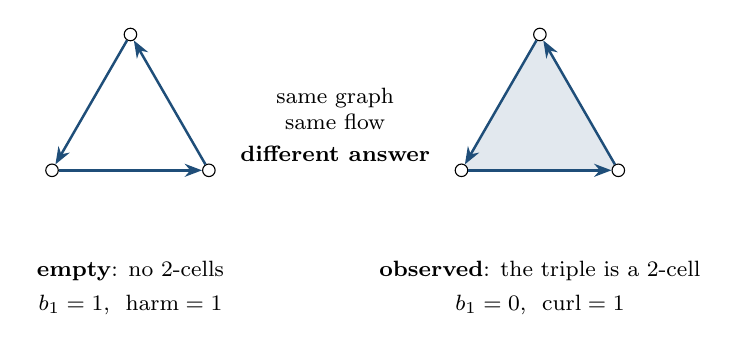
\begin{tikzpicture}[scale=1.0,
  every node/.style={font=\small},
  vtx/.style={circle,draw,fill=white,inner sep=1.6pt},
  flow/.style={-{Stealth[length=2.2mm]},line width=.9pt,color=NavyLink}]
\begin{scope}
  \node[vtx] (a) at (90:1.15) {};
  \node[vtx] (b) at (210:1.15) {};
  \node[vtx] (c) at (330:1.15) {};
  \draw[flow] (a) -- (b); \draw[flow] (b) -- (c); \draw[flow] (c) -- (a);
  \node[font=\footnotesize] at (0,-1.85) {\textbf{empty}: no 2-cells};
  \node[font=\footnotesize] at (0,-2.28) {$b_1 = 1$, \ $\harm = 1$};
\end{scope}
\begin{scope}[xshift=5.2cm]
  \fill[NavyLink,opacity=.13] (90:1.15) -- (210:1.15) -- (330:1.15) -- cycle;
  \node[vtx] (a2) at (90:1.15) {};
  \node[vtx] (b2) at (210:1.15) {};
  \node[vtx] (c2) at (330:1.15) {};
  \draw[flow] (a2) -- (b2); \draw[flow] (b2) -- (c2); \draw[flow] (c2) -- (a2);
  \node[font=\footnotesize] at (0,-1.85) {\textbf{observed}: the triple is a 2-cell};
  \node[font=\footnotesize] at (0,-2.28) {$b_1 = 0$, \ $\curl = 1$};
\end{scope}
\node[font=\footnotesize,align=center] at (2.6,0)
  {same graph\\same flow\\[2pt]\textbf{different answer}};
\end{tikzpicture}
\caption{Filling is a modelling choice, not a property of the data. One
circulating flow on one triangle reads as pure harmonic when no triple is
declared a $2$-cell, and as pure curl when it is. Measured: $\harm = 1.000$,
$b_1 = 1$ against $\curl = 1.000$, $b_1 = 0$. Every result in this document
therefore names its filling.\label{fig:filling}}
\end{figure}

\paragraph{Magnitude, not sign.} A $\pm 1$ sign flow of even a perfectly
transitive order is \emph{not} a pure gradient: the quantisation deposits
spurious harmonic mass. We measured $\harm = 0.200$ at $n=5$ and $\harm=0.2222$
at $n=6$ on a complete graph under the empty filling. The value is
$n$-dependent, which is itself worth stating --- an early draft of our
specification quoted $0.200$ as a constant. Consequently every flow intended to
represent a magnitude uses value-differences or log-odds; sign encodings are used
only to read a tournament for triad statistics.

\section{Known-answer construction}

The rig manufactures data from two vertex populations: integers, which carry a
genuine total order, and complex numbers on the unit circle, which carry none
($\mathbb{C}$ is not an orderable field). Edges fall into three blocks with
deliberately chosen signatures, and the design keeps three distinct sources of
harmonic mass separable, since conflating them is precisely how a certificate
acquires a false positive.

\begin{table}[h]
\centering
\small
\begin{tabular}{@{}lll@{}}
\toprule
\textbf{Source} & \textbf{Generator} & \textbf{Behaviour under more data} \\
\midrule
Systematic & complex--complex rotational rule & persists --- \emph{this is the signal} \\
Innocent null & sparse noisy BTL on comparable items & decays to a floor \\
Incomparability & integer--complex ``bridge'' & depends on mode \\
\bottomrule
\end{tabular}
\caption{The three sources, kept apart by construction.}
\end{table}

\subsection{The oracles}

Each construction is chosen so its decomposition is known analytically. These are
not regression baselines recorded from a previous run; they are values derived
independently of the code, which the code must reproduce.

\begin{table}[h]
\centering
\small
\begin{tabular}{@{}llr@{}}
\toprule
\textbf{Construction} & \textbf{Predicted} & \textbf{Measured} \\
\midrule
Integer pool, value-difference flow & $\harm = 0$, both fillings & $0.000000$ \\
Equal-spaced complex, empty filling & $\harm = 1$, $\grad = 0$ & $1.000000$ \\
Equal-spaced complex, observed filling & $\curl = 1$, $\harm = 0$ & $1.000000$ \\
Complex-only, empty: $b_1$ & $(m{-}1)(m{-}2)/2$ & exact, $m\in\{3,5,7,9\}$ \\
Misspecified null floor & $\varepsilon^2$ & $0.010000$, $0.040000$, $0.160000$ \\
Potential-consistent bridge & $=$ C--C floor exactly & $10.0000$ vs.\ $10.0000$ \\
\bottomrule
\end{tabular}
\caption{Known answers and the values the instrument returns.}
\end{table}

The equal-spaced complex construction deserves comment. Placing $m$ points at
angles $2\pi k/m$ and orienting each edge by the rotational rule gives a
divergence-free flow, hence pure harmonic under the empty filling and pure curl
under the observed one. It is simultaneously the cleanest adversarial signal
available and a direct demonstration that the curl/harmonic split is a modelling
choice rather than a property of the data.

\subsection{The bridge must be potential-consistent}\label{subsec:bridgepc}

The integer--complex bridge admits no natural rule, so it is a configuration
axis: a coin flip drawn fresh per comparison (variance, decaying), a coin flip
drawn once per pair (a persistent random field), or a deterministic surrogate
order. The third case carries a subtlety worth recording. For the surrogate
bridge to contribute \emph{no} harmonic mass, it must be the gradient of the same
potential the integer block is generated from,
\[
Y[i,c] \;=\; s[c] - s[i], \qquad s[c] = \min_i s[i] - \text{gap},
\]
rather than a constant offset. A constant bridge is a global gradient only when
the integer block is flat; against a sloped block it is no longer $D_0 s$ for any
$s$ and deposits harmonic of its own. Measured on $n_{\mathrm{int}}=6$,
$n_{\mathrm{cplx}}=5$: the potential-consistent bridge reads $10.0000$, equal to
the complex block alone to machine precision, while a constant bridge reads
$57.7273$.

\section{The null, and why it must be injected}

The natural null is a Bradley--Terry latent with a genuine total order, observed
on a sparse graph with $k$ comparisons per edge. It does not work, for a reason
that is instructive.

\begin{observation}[The exact null has floor exactly zero]
For any latent potential $\theta$, the clean-limit flow $D_0\theta$ is a pure
gradient, so $\Ph D_0\theta = 0$ identically. Measured:
$\|\Ph D_0\theta\|^2 \approx 1.7\times 10^{-13}$ for every
$\gamma\in\{1,1.5,2,3,6\}$ of a shape family we swept.
\end{observation}

This retired an entire axis of our design. We had expected the shape of $\theta$
--- specifically its asymmetry --- to govern whether a ``logit-bias floor''
survived infinite data, and had built a continuous asymmetry parameter to probe
it. The identity says no shape can produce a budget-independent floor, because
the projector annihilates \emph{every} gradient. Under the exact null, harmonic
mass is pure finite-$k$ estimation error and vanishes as $k\to\infty$; calibrating
a threshold on it would recover zero and validate nothing.

The floor the certificate must not false-flag comes instead from mild
\emph{misspecification}: a criterion that is mostly rankable but whose latent
log-odds surface carries a small non-gradient component surviving infinite data.
We generate it directly and by known amount. On the fixed edge set, let $h$ be a
unit harmonic direction of that graph and filling, and set
\begin{equation}
\text{latent} \;=\; D_0\theta \;+\; \varepsilon\, h ,
\qquad p_e = \sigma(\text{latent}),
\label{eq:inject}
\end{equation}
then sample $k$ Bernoulli comparisons per edge. Because $\Ph h = h$ and
$\Ph D_0\theta = 0$, the budget-independent floor is exactly $\varepsilon^2$ ---
a known answer for the very quantity being calibrated, and the pivot of the whole
method. Setting $\varepsilon=0$ recovers the exact null as a negative control,
whose floor must come out indistinguishable from zero.

\begin{figure}[h]
\centering
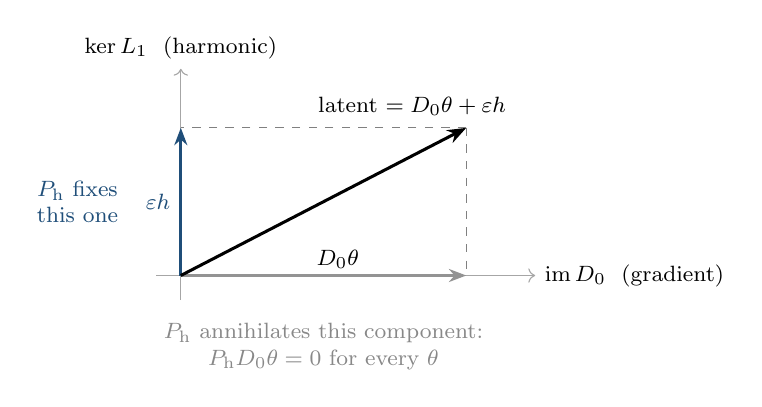
\begin{tikzpicture}[scale=1.25,every node/.style={font=\small}]
  \draw[->,gray!70] (-0.25,0) -- (3.6,0)
     node[right,font=\footnotesize,black] {$\mathrm{im}\,D_0$ \ (gradient)};
  \draw[->,gray!70] (0,-0.25) -- (0,2.1)
     node[above,font=\footnotesize,black] {$\ker L_1$ \ (harmonic)};
  \draw[-{Stealth[length=2.2mm]},line width=1pt,gray!85] (0,0) -- (2.9,0)
     node[pos=.55,above,font=\footnotesize,black,inner sep=2pt] {$D_0\theta$};
  \draw[-{Stealth[length=2.2mm]},line width=1pt,NavyLink] (0,0) -- (0,1.5)
     node[midway,left,font=\footnotesize] {$\varepsilon h$};
  \draw[-{Stealth[length=2.4mm]},line width=1.1pt,black] (0,0) -- (2.9,1.5);
  \node[font=\footnotesize,align=left] at (2.35,1.72) {latent $= D_0\theta + \varepsilon h$};
  \draw[dashed,gray] (2.9,1.5) -- (0,1.5);
  \draw[dashed,gray] (2.9,1.5) -- (2.9,0);
  \node[font=\footnotesize,color=RuleGrey,align=center] at (1.45,-0.72)
     {$\Ph$ annihilates this component:\\$\Ph D_0\theta = 0$ for every $\theta$};
  \node[font=\footnotesize,color=NavyLink,align=center] at (-1.05,0.75)
     {$\Ph$ fixes\\this one};
\end{tikzpicture}
\caption{Why the floor is injected rather than inherited. For \emph{any}
potential $\theta$ the clean-limit flow $D_0\theta$ lies wholly in the gradient
subspace, so $\Ph D_0\theta = 0$ and no choice of $\theta$ --- however skewed
--- leaves harmonic mass behind. Adding $\varepsilon h$ along a unit harmonic
direction gives $\|\Ph(\text{latent})\|^2 = \varepsilon^2$ exactly: a known
answer for the quantity being calibrated.\label{fig:inject}}
\end{figure}

\section{Estimation}\label{sec:estimation}

\subsection{The model}

Expanding the harmonic energy of the observed log-odds flow,
\begin{equation}
\mathbb{E}\,\|\Ph Y\|^2
\;=\; \underbrace{\|\Ph\,\text{bias}\|^2}_{=\;\varepsilon^2}
\;+\; \frac{\tr(\Ph \Sigma)}{k} \;+\; O(k^{-2})
\;=\; \text{floor} + \frac{c}{k} + O(k^{-2}).
\label{eq:model}
\end{equation}
The variance term is predictable rather than a fitted nuisance: by the delta
method on $\mathrm{logit}(\hat p_e)$,
\begin{equation}
c \;=\; \tr\!\Big(\Ph \cdot \operatorname{diag}\big(1/(p_e(1-p_e))\big)\Big),
\label{eq:coracle}
\end{equation}
which gives an independent check on the fit. Equation~\eqref{eq:coracle} is not
the whole $O(k^{-1})$ coefficient. The plug-in estimator $\mathrm{logit}(\hat
p_e)$ is a raw clamped logit --- the $1/(2k)$ clamp binds only at $w\in\{0,k\}$,
with probability below $10^{-13}$ across the fit window, so it is not a
continuity correction --- and therefore carries its mean bias
$b_e=(2p_e-1)/\bigl(2p_e(1-p_e)\bigr)$ at order $k^{-1}$ in full. Expanding
$\|\Ph\mathbb{E}[Y]\|^2$ rather than $\mathbb{E}\|\Ph Y\|^2$ leaves a cross term
beside it, and because $\Ph\lambda = \varepsilon h$ exactly it collapses to a
scalar with no projector left in it:
\begin{equation}
c_1 \;=\; \tr(\Ph V) \;+\; 2\varepsilon\,\langle h, b\rangle,
\qquad V=\operatorname{diag}\big(1/(p_e(1-p_e))\big).
\label{eq:c1}
\end{equation}
Computed on exact binomial energies rather than sampled ones,
\eqref{eq:c1} reproduces the measured $O(k^{-1})$ coefficient to eight decimal
places on both calibration topologies, while \eqref{eq:coracle} alone is short by
$4.5\%$ and $0.2\%$. The cross term therefore \emph{completes} the delta-method
oracle rather than refining it, and there is no further $O(k^{-1})$
contribution: an earlier reading of this gap as one was an artefact of estimating
$c$ with a two-parameter fit on sampled energies, which absorbs part of the
$O(k^{-2})$ term treated in \S\ref{subsec:window}. We keep \eqref{eq:coracle} as
the shipped predictor, since it is what the guard was calibrated against and what
the derived window uses. Model \eqref{eq:model} is linear in
$(\text{floor}, c)$ under $x = 1/k$, so the floor is simply the intercept of an
ordinary least-squares line, fitted per seed --- the graph, and hence $\Ph$ and
the true floor, are held fixed within a seed --- and aggregated across seeds.

\subsection{Two constraints that are not optional}

\paragraph{Standardise the latent across shape.} When sweeping the latent's shape
we hold its standard deviation fixed. Without this, changing shape also changes
signal strength, and the two are confounded along the one axis meant to isolate
shape.

\paragraph{Hold the graph fixed across the $k$-sweep.} The floor
$\|\Ph\,\text{bias}\|^2$ is a function of the graph, and $\Ph$ moves with the
edge set. If the sparsity mask were redrawn per $k$, the floor would not be
constant across the sweep and \eqref{eq:model} would not be a well-posed fit. The
mask is drawn once per seed; only the Bernoulli outcomes vary with $k$.

\subsection{The fit window, and why it is derived}\label{subsec:window}

The $O(k^{-2})$ term in \eqref{eq:model} is not negligible at small $k$, and a
two-parameter fit absorbs it into the intercept. Fitting the full grid biases the
floor by factors of $0.83$ to $2.48$ depending on separation --- on the graph of
Figure~\ref{fig:window} an intercept of $0.186$ against a true floor of $0.090$,
where the windowed fit gives $0.084$. Adding $c_2/k^2$ as a \emph{free} third
parameter is worse, not better --- on sampled energies it is poorly conditioned
and eats the intercept. What that objection assumed, and what \S\ref{sec:results}
retires, is that $c_2$ is unknown. It is not: it has a closed form in the null
the rig already constructs, so the leak can be removed by subtracting a known
quantity rather than by spending a parameter to recover it. Discarding the
contaminated points remains the cheaper option; subtracting $c_2$ is the option
when the last tenth of a percent matters.

Our first formulation declared a constant, $k \geq 64$. That was calibrated under
the observed filling and is wrong under any filling with a different $c$. On one
graph:

\begin{table}[h]
\centering
\small
\begin{tabular}{@{}lrrrr@{}}
\toprule
\textbf{Filling} & $b_1$ & $c$ & \textbf{floor at $k\!\geq\!64$} & \textbf{true} \\
\midrule
observed & $2$  & $18$  & $0.0807$ & $0.090$ \\
empty    & $20$ & $160$ & $0.0156$ & $0.090$ \\
\bottomrule
\end{tabular}
\end{table}

\begin{figure}[h]
\centering
\includegraphics[width=.86\textwidth]{fig-window.pdf}
\caption{The floor is an intercept, so which points the fit may use decides it.
Ten measured energies from one graph at $\varepsilon=0.3$. Model
\eqref{eq:model} is a straight line in $1/k$; fitting all of them lets the
small-$k$ end, where the $O(k^{-2})$ term lives, dominate the least squares.
Same data, same estimator, one decision.\label{fig:window}}
\end{figure}

\noindent
The window is therefore derived per configuration from quantities already
available in closed form,
\begin{equation}
k_{\min} \;=\; \frac{c}{\rho \cdot \text{floor}},
\label{eq:window}
\end{equation}
where $\rho$ is a resolvability margin: at $k_{\min}$ the variance term equals
$\rho$ times the floor being resolved --- its largest value among the retained
points, so a smaller $\rho$ keeps only cleaner, higher-$k$ data. A grid that cannot reach
$k_{\min}$ is flagged and \emph{not fitted}. Deriving the window dissolves the
filling dependence --- both fillings recover given a grid that reaches the
requirement --- and removed most of a residual bias we had been carrying as an
unexplained constant.

\section{Guard discipline}

Three rules govern how the estimator fails.

\paragraph{Check preconditions in closed form, before fitting.} Model
\eqref{eq:model} holds in a bounded region. At extreme separation the log-odds
estimator saturates: with $p_e$ near $0$ or $1$, wins land at $0$ or $k$, the
clamp forces $Y = \mp\log(2k-1)$, and the distortion \emph{grows} as $\log 2k$
instead of decaying. Saturation is computable without sampling as
$\mathbb{E}_e[p_e^{k} + (1-p_e)^{k}]$, so it is checked first and the fit is
refused outside the window. A loud failure is the correct output; a floor number
is not.

\paragraph{A guard may be necessary without being sufficient.} The delta-method
prediction \eqref{eq:coracle} is a genuine misspecification detector. It caught a
default separation parameter of ours that saturated the clamp: the fitted floor
read $0.2591$ against a true $0.0900$ --- an entirely plausible number --- and
only the disagreement between fitted $c=9.44$ and predicted $c=70.07$ revealed
the fit as misspecified rather than informative. But the same guard reads
$c_{\mathrm{fit}}/c_{\mathrm{oracle}} = 1.01$, essentially exact, at a separation
where the floor is still $1.86\times$ too high. It is necessary and not
sufficient, and we say so wherever it appears. Reporting it as \emph{the} gate
would have licensed exactly the errors it cannot see. Figure~\ref{fig:guard}
shows the blind spot as a region rather than an anecdote, and shows that
improving the estimator moved it without closing it: under the tuned
configuration a case remains where the floor is recovered at $0.05\times$ its
true value --- twenty times too small --- while the guard reads $1.00$.

\begin{figure}[h]
\centering
\includegraphics[width=\textwidth]{fig-guard.pdf}
\caption{The guard's blind spot. Each point is a configuration; the green band
is where the $c$-check passes, the grey band where the floor is actually
correct. Points in the green band but outside the grey one are the failures the
guard cannot see. Tuning the estimator (right) removed most bad configurations
but not the blind spot itself --- and made its worst case more extreme, not
less.\label{fig:guard}}
\end{figure}

\paragraph{Distinguish degradation from destruction.} When emitting synthetic
judgement logs, a target flow whose magnitude falls inside the representable band
around zero legitimately rounds to a tie; that is quantisation loss, reported as
a residual. A flow that quantises to zero \emph{entirely} is not rounding, it is
emitting nothing, and raises. Both failure modes produce a well-formed
decomposition rather than an exception, which is exactly what makes them
dangerous --- nothing downstream can tell that the number it received is
meaningless.

\section{Reporting discipline}

\begin{principle}[Seed-varying quantities ship with their spread]
Any figure that moves with the seed is reported as a distribution --- mean,
standard error, and per-draw range over independent base seeds. A single run's
value is a draw, not the quantity.
\end{principle}

We arrived at this by getting the same number wrong three times. A residual bias
was reported as ``$\sim$10\%'', then ``3--6\%'', then ``$\sim$2.0--2.4\%'';
coverage of the oracle by the confidence interval as ``16/20'', then ``15/16''.
Each was a single draw, each was superseded by the next, and each \emph{looked}
settled because nothing in the output marked it as variable. Re-measured over
$20$ independent base seeds the residual was $1.6\% \pm 0.2\%$ and coverage was
\emph{typically} $13/16$ --- so ``15/16'', reported twice as the result, had been
the best of twenty draws.

\begin{figure}[h]
\centering
\includegraphics[width=.86\textwidth]{fig-draws.pdf}
\caption{Twenty independent base seeds of the same quantity, with the three
figures we successively reported as \emph{the} result marked below. Each was a
legitimate draw; none was the quantity. The spread is wide enough that a single
run supports almost any of them --- but the spread is Monte Carlo. The same
quantity computed with exact energies is $+0.3624\% \pm 0.0024\%$, a per-draw
range of $0.046$ pt against the $1.685$ pt plotted here. The three figures are
draws from the sampling law, not from the estimator.\label{fig:draws}}
\end{figure}

The mechanism that exposed it is worth stating because it recurs: adding one
field to the configuration changed the configuration's hash, the seed derivation
consumes that hash, so every graph reseeded and settled-looking numbers moved.
Accordingly each record also carries the full budget that produced it --- seed
count, replication, grid, window parameters --- so that no number can be read
without the conditions that generated it, and the same configuration and seed
reproduce byte-identical output.

\section{Validation protocol}

Acceptance is defined as a numbered list of claims, each with a test that
exercises it against the real instrument. The current suite is $70$ tests in
$4.5$ seconds, fast enough to run on every edit. Three features are deliberate.

\emph{Negative controls carry equal weight.} $\varepsilon=0$ must yield a floor
whose interval covers zero; the symmetric latent shape must yield a floor
indistinguishable from any other shape's.

\emph{Traps are permanent regression tests.} Each defect found becomes a test
asserting the trap still bites: the sign-quantisation bias with its
$n$-dependence, the single-row emission that produces an identically zero flow,
the constant bridge that breaks the potential-consistency identity.

\emph{Known exceptions are strict.} Where a claim is known to fail in a specific
cell, it is recorded as a strict expected-failure rather than by widening a
tolerance. This is not decoration: when a later change closed the gap, the strict
marker converted the pass into a failure and forced the stale exemption to be
deleted rather than carried on unexamined. A widened tolerance would have
absorbed the improvement silently.

\section{Results}\label{sec:results}

The instrument reproduces every known answer (Table 2). The synthetic adversarial
sweep behaves as predicted: with equal spacing every complex--complex edge
carries unit harmonic energy under the empty filling, so the systematic floor
follows $m(m-1)/2$ exactly --- measured $0, 3, 10, 21, 36$ --- while the raw
harmonic \emph{fraction} over the same sweep moves only $0.004$ to $0.092$,
diluted by blocks of differing per-edge energy. We therefore state the
monotonicity claim on the floor and report the fraction alongside, so the
confound stays visible rather than being quietly resolved in our favour.

The triad statistic behaves as the certificate's motivation requires. On a
$4$-cycle beside a transitive triangle, the coefficient of consistency sees only
the triple it can, finds it perfectly transitive, and reports $1.0$ --- while a
third of the flow's energy is harmonic and unrankable.

Tuning the resolvability margin $\rho$ closed most of the remaining bias. The
residual falls monotonically as $\rho$ falls, because a smaller $\rho$ demands a
longer and cleaner tail; lower $\rho$ costs grid reach, so $\rho$ and the grid
must be tuned together.

\begin{table}[h]
\centering
\small
\begin{tabular}{@{}lrrr@{}}
\toprule
\textbf{Configuration} & \textbf{Residual} & \textbf{Coverage} & \textbf{Unfittable cells} \\
\midrule
$\rho = 3.0$, grid to $4096$   & $+1.6\% \pm 0.2\%$   & median $13/16$ & $0.17$ \\
$\rho = 1.5$, grid to $16384$  & $+0.43\% \pm 0.09\%$ & median $15/16$ & $0.00$ \\
\bottomrule
\end{tabular}
\caption{Over $20$ independent base seeds; per-draw spread tightened from
$(-0.7\%, +3.4\%)$ to $(-0.52\%, +1.16\%)$.\label{tab:rho}}
\end{table}

A bias of $+0.43\% \pm 0.09\%$ survives both levers, and neither margin nor grid
length removes it --- because neither addresses it. The residual is not an
unexplained constant but the $O(k^{-2})$ term of \eqref{eq:model} leaking into a
two-parameter intercept. Over any window of positive $x=1/k$ the omitted
$c_2/k^2$ projects onto the constant and biases the fitted intercept low, by the
amount the residual measures.

Two facts fix what $c_2$ is. The mean bias $b$ that completes the $O(k^{-1})$
coefficient in \eqref{eq:c1} is nearly irrelevant here: expanding both the mean
and the variance to second order gives
$c_2 = \langle b,\Ph b\rangle + 2\varepsilon\langle h,b_2\rangle + \sum_e
(\Ph)_{ee}\,v_2(p_e)$, and the composition is $95$--$99\%$ the third term, with
$\langle b,\Ph b\rangle$ contributing about $1\%$. The expectation that whatever
drives the $1/k$ correction also drives the $1/k^2$ one is wrong by two orders of
magnitude. The term that does drive it is the second-order \emph{variance} of the
logit, in closed form
\begin{equation}
v_2(p) \;=\; \frac{2}{pq} \;+\; \frac{3}{2}\cdot\frac{(2p-1)^2}{(pq)^2},
\qquad q = 1-p,
\label{eq:v2}
\end{equation}
confirmed against exact binomial moments and independently by a third-order delta
method, in which the $2/(pq)$ piece is the near-boundary $g'g'''$ tail.

Computed with exact energies over $20$ base seeds --- no Monte Carlo --- the
residual is $+0.3624\% \pm 0.0024\%$. Two consequences follow. First, the shipped
$\pm 0.09$ pt band was almost entirely $\texttt{reps}=16$ sampling noise rather
than base-seed variation: the underlying quantity is near-deterministic, and its
standard error is some forty times narrower than the sampled figure it explains.
Second, the residual grows with $\varepsilon$ as part of the same mechanism, not
separately --- the derived window $k_{\min} = \tr(\Ph V)/(\rho\varepsilon^2)$
admits lower-$k$ points as $\varepsilon$ rises, so larger-$\varepsilon$ cells fit
nearer the region where $c_2/k^2$ is largest.

Three computations confirm the attribution, all exact on both sides. Subtracting
the closed-form $c_2$ before the two-parameter fit moves the residual to
$+0.0791\% \pm 0.0010\%$; fitting $c_2$ as a third parameter moves it to
$-0.0088\% \pm 0.0004\%$; and changing the edge estimator moves the residual in
the proportion its $c_2$ moves. A per-edge continuity-corrected estimator
$\mathrm{logit}\big((w+\tfrac12)/(k+1)\big)$ has $v_2^F = \tfrac12
(2p-1)^2/(pq)^2$ --- it annihilates the $2/(pq)$ boundary term of \eqref{eq:v2}
outright --- giving $21.19\%$ of the raw $c_2$ on this topology and $22.75\%$ of
the raw residual, agreement to under $2$ pp. That estimator is used here only as
a diagnostic probe, and only per edge; it is not Firth-penalised Bradley--Terry
on the joint design, whose penalty does not factorise over edges and which we
have not tested.

No universal reduction factor exists, which is itself the point:
$v_2^F/v_2$ runs from $0$ at $p=\tfrac12$ to $\tfrac13$ as $p\to 0$, so the
corrected-to-raw $c_2$ ratio is bounded in $(0,\tfrac13)$ and set by the
$\Ph$-weighted edge-probability mix --- $5.2\%$ on a mid-range topology against
$21.2\%$ on one whose edges reach $p\approx0.08$. The mechanism is universal; its
magnitude is topological, as \S\ref{sec:scope} would predict.

The direction is unchanged and remains the conservative one: the floor is
under-read, so a threshold calibrated from it sits slightly low, biasing toward
false alarms rather than missed detections. For an instrument whose purpose is
detecting non-rankability, that is the direction in which to be wrong.

\section{Scope: the threshold is topology-bound}\label{sec:scope}

The most consequential limit the method establishes is not a defect but a fact
about the object.

\begin{observation}[$b_1$ is non-monotone in the item count]
Under the observed filling at fixed edge retention $0.45$, the fraction of
graphs with $b_1 = 0$ falls from $64.7\%$ at $n=6$ to a minimum of $11.4\%$ at
$n=12$, then \emph{rises} again --- $21.6\%$ at $n=18$, $44.8\%$ at $n=24$,
$64.2\%$ at $n=28$. Mean $b_1$ peaks at $n=14$ and decays thereafter.
\end{observation}

\noindent
The mechanism is immediate once seen: at fixed retention, more items means more
\emph{observed triples}, and filling them destroys the very holes the
certificate reads. Beyond the optimum, collecting more items reduces the
instrument's sensitivity toward zero. We had originally recorded this as a
plateau, on evidence that stopped at $n=14$; extending the sweep showed the
rise. Figure~\ref{fig:rho} shows both this curve and the $\rho$ trade-off.

The rise beyond the optimum is the expected asymptotics of the object, not an
artefact of the sweep. Under the observed filling the complex is the
two-skeleton of the random flag complex on $G(n,p)$, whose first homology has a
sharp vanishing threshold in the edge density that tends to zero as
$n \to \infty$~\cite{kahle2014}. Any fixed retention eventually exceeds it,
forcing $b_1 \to 0$: past some item count, collecting more data provably removes
the structure the certificate reads, not merely fails to add to it.\footnote{The
asymptotic exponent is not yet visible at the sizes swept here. Bisecting for the
retention $p^{*}$ at which $\Pr[b_1 = 0]$ crosses $1/2$ gives $0.595$, $0.581$,
$0.515$, $0.475$, $0.449$, $0.429$ at $n = 8, 12, 16, 20, 24, 30$ --- a fitted
decay of $n^{-0.27}$ against the asymptotic $n^{-1/2}$, with $p^{*}/n^{-1/2}$
drifting monotonically from $1.68$ to $2.35$. The threshold is decaying as the
theory requires; the exponent has not converged. This cuts the useful way
operationally: at realistic $n$ the usable window is \emph{wider} than the
asymptotic form suggests, so the constraint should be evaluated at the deployment's
own $(n,p)$ rather than from the limit.}

\begin{figure}[h]
\centering
\includegraphics[width=\textwidth]{fig-rho-plateau.pdf}
\caption{Left: the residual falls monotonically as the resolvability margin
$\rho$ falls, because a smaller $\rho$ demands a longer, cleaner tail --- but
cells become unfittable as the grid stops reaching the required window, so the
two must be tuned together. Right: the $b_1=0$ rate against item count at fixed
edge retention. There is an interior optimum; past it, more items destroy the
holes.\label{fig:rho}}
\end{figure}

The same fact appeared independently as the filling dependence of the fit window
(\S\ref{subsec:window}), where a constant calibrated under one topology under-read the floor by
$6\times$ under another. These are one object, and the non-monotonicity sharpens
it: not only does scaling the item count fail to fix topology dependence, past
an optimum it actively removes the structure being measured. Since $\Ph$ is determined by the
comparison graph, so are the floor, the variance coefficient $c$, and any
threshold derived from them.

\begin{principle}[No universal threshold]\label{prin:nouniversal}
A null calibrated on one topology does not transfer to another. The deliverable
is not a number but a procedure: given a deployment's own comparison graph,
generate the matched null and derive the window on it --- recomputed whenever the
comparison \emph{pattern} changes, not only when the item set does.
\end{principle}

The derived window of \S\ref{subsec:window} is the template for this at one level down. The
failure it corrects --- a constant calibrated under one topology, silently wrong
under another --- is precisely the failure a transferred threshold would make.

\section{What the method does not establish}

The rig validates the instrument, not the judge. Nothing here shows that a
language-model comparator's harmonic deviation is interpretable; it shows that
\emph{if} such a deviation is measured, the measurement machinery is sound and
two synthetic reference lines exist to read it against --- a comparator that
thrashes on incomparable pairs deposits variance that washes out with
replication, one that fabricates a surrogate order deposits none at all. Whether
a real comparator resembles either is the next question, and it is now the only
thing standing between this method and its intended use.

A second gap is narrower but concrete. The rig calibrates its null at the true
edge probabilities, which it knows by construction; a deployment knows only the
data it is judging and must estimate the null from it. That estimate carries a
modelling choice the rig never faces --- which flows the fitted null is permitted
to contain. A null fitted as a pure gradient (a Bradley--Terry fit) assumes the
criterion is rankable before testing whether it is, and misstates the harmonic
band wherever the comparator carries genuine local inconsistency on the edges a
hole runs through; a null fitted to the gradient-and-curl subspace does not.
Choosing that subspace is part of generating the matched null
Principle~\ref{prin:nouniversal} already requires, and it has to be stated rather
than defaulted.

\begin{thebibliography}{9}
\bibitem{jiang2011}
X.~Jiang, L.-H.~Lim, Y.~Yao, and Y.~Ye.
\newblock Statistical ranking and combinatorial Hodge theory.
\newblock \emph{Mathematical Programming}, 127(1):203--244, 2011.

\bibitem{kahle2014}
M.~Kahle.
\newblock Topology of random simplicial complexes: a survey.
\newblock In \emph{Algebraic Topology: Applications and New Directions},
volume 620 of \emph{Contemporary Mathematics}, pages 201--221. American
Mathematical Society, 2014. \newblock arXiv:1301.7165.

\bibitem{kendall1940}
M.~G.~Kendall and B.~Babington Smith.
\newblock On the method of paired comparisons.
\newblock \emph{Biometrika}, 31(3/4):324--345, 1940.

\bibitem{bradley1952}
R.~A.~Bradley and M.~E.~Terry.
\newblock Rank analysis of incomplete block designs: I. The method of paired
comparisons.
\newblock \emph{Biometrika}, 39(3/4):324--345, 1952.
\end{thebibliography}

\end{document}
